\begin{frame}[plain]{Az algoritmus pszeudokódja (PathLabel metódus)}
% \scriptsize
% \begin{algorithmic}
%   \State \nextalgline\ \textbf{procedure} \textsc{PathLabel}$(s, t, e)$

%   \State \nextalgline\ \ \textbf{if} $IN[s] < IN[t] < OUT[s]$ \textbf{then}   \Comment{{s is ancestor of t}}
%   \State \nextalgline\ \ \ \textbf{return}

%   \State \nextalgline\ \ \textbf{if} $IN[t] < IN[s] < OUT[t]$ \textbf{then}  \Comment{{t is ancestor of s}}
%   \State \nextalgline\ \ \ PLAN $\gets$ \textsc{ANCESTOR}; $k_1 \gets IN[t]$; $k_2 \gets IN[s]$
%   \State \nextalgline\ \textbf{else}
%   \State \nextalgline\ \ \ \textbf{if} $IN[s] < IN[t]$ \textbf{then}
%   \State \nextalgline\ \ \ \ \ PLAN $\gets$ \textsc{LEFT}; $k_1 \gets OUT[s]$; $k_2 \gets IN[t]$
%     \Comment{{s is left of t}}
%   \State \nextalgline\ \ \ \textbf{else}
%   \State \nextalgline\ \ \ \ \ PLAN $\gets$ \textsc{RIGHT}; $k_1 \gets OUT[t]$; $k_2 \gets IN[s]$
%     \Comment{{s is right of t}}

%   \State \nextalgline\ $v \gets s$

%   \State \nextalgline\ \textbf{while} $k_1 < k_2$ \textbf{do}     \Comment{{Detecting when below LCA(s, t)}}

%   \State \nextalgline\ \ \ \textbf{if} \textsc{find}$(v) = v$ \textbf{then}   \Comment{{If true, set replacement edge for (v, P[v])}}
%   \State \nextalgline\ \ \ \ \ $R(v, P[v]) \gets e$   \Comment{{Set the replacement edge}}
%   \State \nextalgline\ \ \ \ \ \textsc{link}$(v)$   \Comment{{Union the disjoint sets of $v$ and $P[v]$}}

%   \State \nextalgline\ \ \ $v \gets \textsc{find}(v)$

%   \State \nextalgline\ \ \ \textbf{switch} PLAN \textbf{do}
%   \State \nextalgline\ \ \ \ \ \textbf{case} \textsc{ANCESTOR}:
%   \State \nextalgline\ \ \ \ \ \ $k_2 \gets IN[v]$
%   \State \nextalgline\ \ \ \ \ \textbf{case} \textsc{LEFT}:
%   \State \nextalgline\ \ \ \ \ \ $k_1 \gets OUT[v]$
%   \State \nextalgline\ \ \ \ \ \textbf{case} \textsc{RIGHT}:
%   \State \nextalgline\ \ \ \ \ \ $k_2 \gets IN[v]$

% \end{algorithmic}
  \centering
  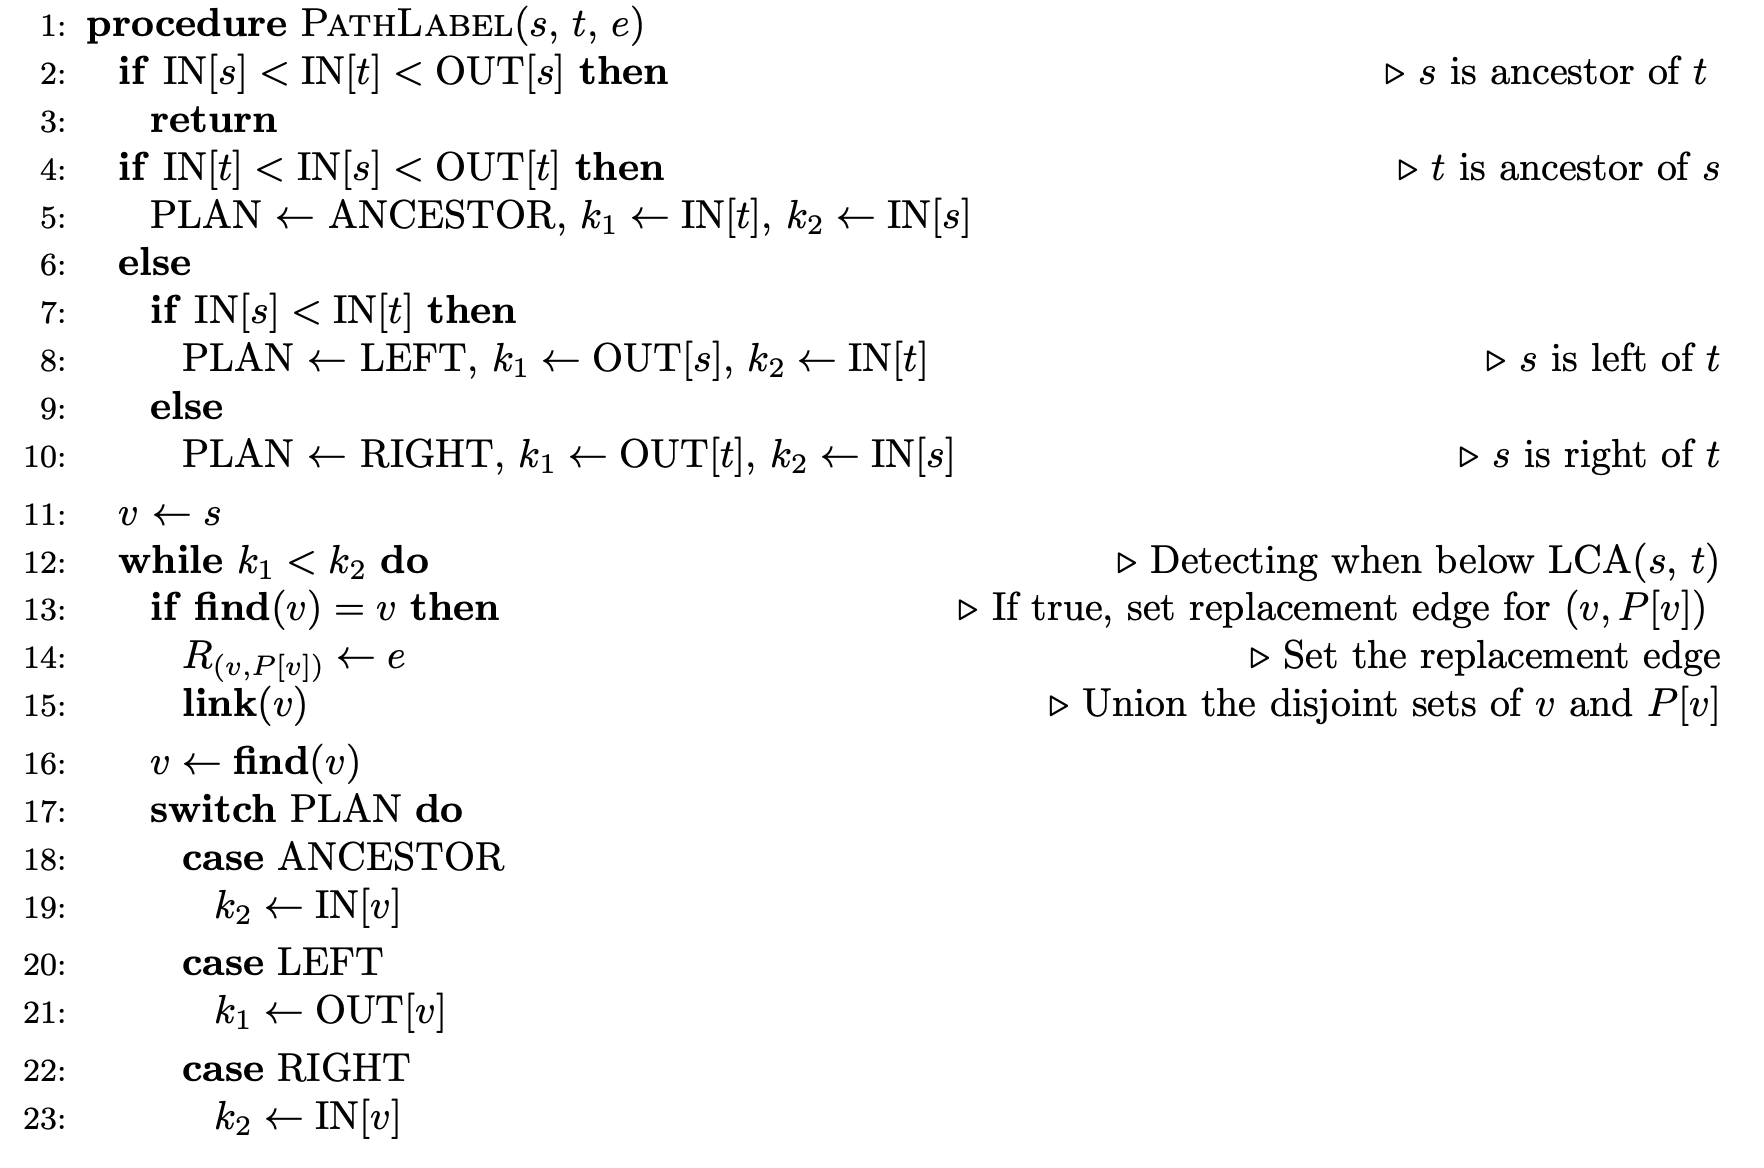
\includegraphics[width=0.8\textwidth]{images/path-label-pseudocode.png}
\end{frame}

\begin{frame}{PathLabel funkciója}
  \begin{itemize}
    \item Meghatározza s és t élek pozícióját egymáshoz képest az MST-n. (LEFT, RIGHT, ANCESTOR)
    \item s éllel kezdve végig megyünk az s $\rightarrow$ t úton, és:
    \begin{itemize}
      \item Ha az adott él még nem volt úttömörítve (v = find(v)), akkor annak az élnek az inputként megadott élet menti el csereélének. Majd úttömörítést hajtunk végre (link(v)).
      \item $k_1$ és $k_2$ counter-eket léptetgeti, ameddig végig nem érünk az s $\rightarrow$ t úton vagy nem el nem érjük s és t legalacsonyabb közös ősét.
    \end{itemize}
  \end{itemize}
  \begin{block}{2. állítás}
    Az algoritmus a nem-MST él által indukált kört leszármazottól ős felé járja be, és megáll a legalacsonyabb közös ősnél (abban az esetben, ha a legalacsonyabb közös ős különbözik s-től és t-től)
  \end{block}
\end{frame}